\PassOptionsToPackage{usenames, dvipsnames}{color}
\documentclass{article}
\usepackage[latin1]{inputenc}
\usepackage{geometry}
\usepackage[T1]{fontenc}
\usepackage[english]{babel}
\usepackage{graphicx}
\usepackage{amsmath}
\usepackage{amssymb}
\usepackage{setspace}
\usepackage{svg}
\usepackage{fancyhdr}
\usepackage{wrapfig}
\usepackage{circuitikz}
\usepackage{subfig}
\usepackage{hyperref}
\usepackage{sidecap}
\usepackage{theorem}
\usepackage{thc}
\usepackage{url}
\usepackage{booktabs}
\usepackage{multirow}
\usepackage{gensymb}
\usepackage{textcomp}
\usepackage{listings} 
\usepackage{braket}
\usepackage{physics}
\usepackage[usenames]{color}
\usepackage{pgfplots}
\usepackage{graphicx}
\usepackage{titling}
\usepackage{color}
\usepackage{relsize}
\usepackage{amsmath}
\usepackage{xcolor} % Required for specifying custom colors
\usepackage{fix-cm} % Allows increasing the font size of specific fonts beyond LaTeX default specifications
\usepackage[protrusion=true,expansion=true]{microtype} % Better typography
\usepackage{graphicx} % Required for including pictures
\usepackage{wrapfig} % Allows in-line images
\usepackage{mathpazo} % Use the Palatino font
\usepackage[T1]{fontenc} % Required for accented characters
\usepackage[nottoc,numbib]{tocbibind}
\usepackage{import}
\usepackage{standalone}
\usepackage{tikz}
\usepackage{tikz-dimline}
\usepackage{amsmath}
\usepackage{stanli}
\pgfplotsset{compat=1.18}

\def\dx{0.3}
\def\dy{0.3333}
\def\x{0}
\def\xx{1}
\def\y{3}

\makeatletter
\g@addto@macro\@floatboxreset\centering
\makeatother

\usetikzlibrary{patterns.meta}
\hypersetup{pdfborder=0 0 0}

\newcommand\mysymb{\scalebox{.3}{(}\raisebox{-1.7pt}{$-$}\scalebox{.3}{)}}

\setlength{\headheight}{15pt}

\geometry{left=3 cm,right=3 cm, top=3.5 cm, bottom=3.5 cm}
\pagestyle{fancy}
\fancyhead[L,C]{}
\fancyhead[R]{Controller Design for Two Dynamic Systems}
\fancyfoot[C]{\thepage}

\makeatletter
\renewcommand\@biblabel[1]{\textbf{#1.}} % Change the square brackets for each bibliography item from '[1]' to '1.'
\renewcommand{\@listI}{\itemsep=0pt} % Reduce the space between items in the itemize and enumerate environments and the bibliography

\renewcommand{\maketitle}{ % Customize the title - do not edit title and author name here, see the TITLE block below
\begin{flushright} % Right align
{\LARGE\@title} % Increase the font size of the title

\vspace{50pt} % Some vertical space between the title and author name

{\large\@author} % Author name
\\\@date % Date

\vspace{40pt} % Some vertical space between the author block and abstract
\end{flushright}
}

%----------------------------------------------------------------------------------------
%	TITLE
%----------------------------------------------------------------------------------------

\title{\textbf{Controller Design for Two Dynamic Systems}\\ % Title
\vspace{2pt}
Final Course Project for ME 450} % Subtitle
\author{\textsc{Liam McGuire, Andrew Schalk} % Author
\bigskip
\\{\textit{Southern Illinois University Edwardsville}}} % Institution
\date{April 26, 2024} % Date

%----------------------------------------------------------------------------------------

\begin{document}
    \thispagestyle{empty}
    \pagenumbering{gobble}
    \maketitle % Print the title section
    \vspace{300pt} % Some vertical space between the abstract and first secti
    %----------------------------------------------------------------------------------------
    %	ESSAY BODY
    %----------------------------------------------------------------------------------------
    \begin{center}
        \rule{15cm}{.35pt}
    \end{center}
    \section*{Abstract}
    This report details the design and theoretical implementation of controllers for two dynamic systems. 
    The first system's dynamic equations are given by the project requirements.
    We are tasked with designing a PID controller to meet certain design requirements. 
    The second is a magnetic levitation system whose equations we derive. 
    For this system, we design a controller simply to stabilize the system.
    The performance characteristics of both compensated systems are analyzed.
    \newpage
    \tableofcontents
    \newpage
    \pagenumbering{arabic}
    \section{Problem 1}
    \subsection{Problem Definition}
    We begin our study by considering the system described by the state-space equations:
    \begin{equation}
        \begin{aligned}
            \dot{x}_1(t)&=-0.313x_1(t)+56.7x_2(t)+0.232u(t)\\
            \dot{x}_2(t)&=-0.0139x_1(t)-0.426x_2(t)+0.0203u(t)\\
            \dot{x}_3(t)&=56.7x_2(t)\\
            y(t)&=x_3(t)
        \end{aligned}
    \end{equation}
    or in matrix form as
    \begin{equation}
        \begin{aligned}
            \dot{\textbf{x}}&=\textbf{Ax}+\textbf{Bu}\\
            \textbf{y}&=\textbf{Cx}
        \end{aligned}
    \label{eqn:state}
    \end{equation}
    where
    \begin{equation}
        \nonumber
        \textbf{x}=
        \begin{bmatrix}
            x_1\\
            x_2\\
            x_3
        \end{bmatrix}
        \textbf{A}=
        \begin{bmatrix}
            -0.313 &56.7& 0\\
            -0.0139& -0.426& 0\\
            0 &56.7& 0
        \end{bmatrix}
        \textbf{B}=
        \begin{bmatrix}
            0.232\\
            0.0203\\
            0
        \end{bmatrix}
        \textbf{C}=
        \begin{bmatrix}
            0&0&1
        \end{bmatrix}
    \end{equation}
    Taking the Laplace transform of (\ref{eqn:state}) and solving for the transfer function \(G(s)=\frac{Y(s)}{U(s)}\), the equation yields
    \begin{equation}
        \begin{aligned}
            G(s)=&\textbf{C}(s\textbf{I}-\textbf{A})^{-1}\textbf{B}\\
            =&\frac{1.151s+0.1774}{s^3+0.739s^2+0.9215s}
        \end{aligned}
    \end{equation}
    The controller for this system will be designed to meet the following requirements for the response to a step input.
    \begin{equation}
        \nonumber
        \begin{aligned}
            P.O.<&10\%\\
            t_r<&2s\\
            t_s<&10s\\
            e_{ss}<&2\%
        \end{aligned}
    \end{equation}
    \subsection{Open-Loop System}
    By inspection of the plant's transfer function, this can be seen to be a type one system.
    A system of this type - with an integrator - will be unstable, as the input is integrated and the output grows towards infinity.
    This can be seen reflected in the pole-zero map of Figure \ref{fig:OpenLoopPoles}. 
    The dominant pole exists at s=0 which implies marginal stability for this system.
    The step response of this system is shown in Figure \ref{fig:OpenLoopResponse}.
    The output is unstable but the response satisfies the requirement for $T_r$.
    \begin{figure}[ht]
        \centering
        \begin{minipage}{.5\textwidth}
            \includegraphics[scale=.5]{OpenLoopPoles.eps}
            \caption{Open-Loop Pole-Zero Map}
            \label{fig:OpenLoopPoles}
        \end{minipage}%
        \begin{minipage}{.5\textwidth}
            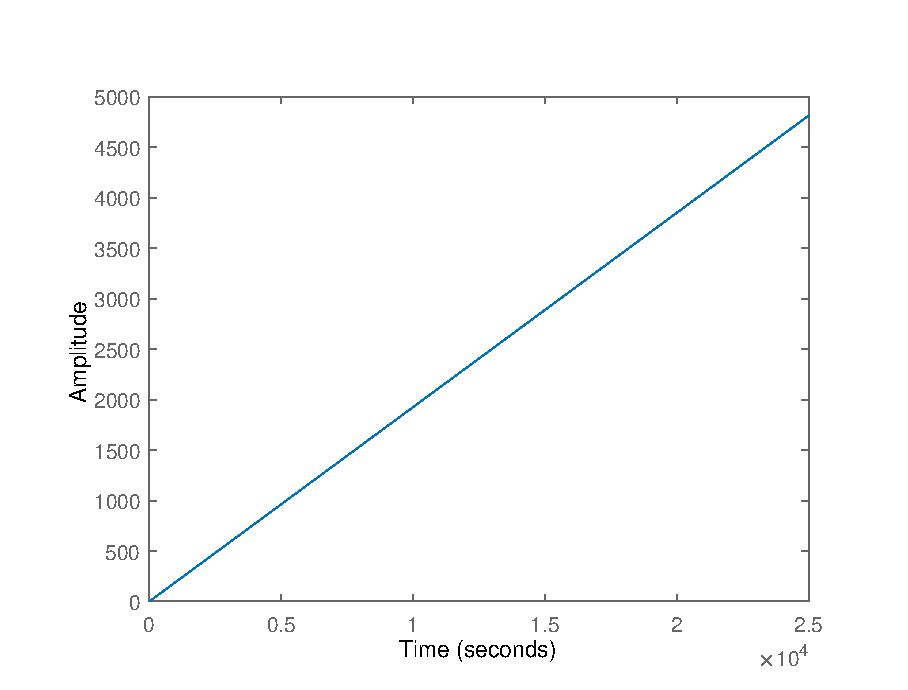
\includegraphics[scale=.5]{OpenLoopResponse.eps}
            \caption{Open-Loop Step Response}
            \label{fig:OpenLoopResponse}
        \end{minipage}
    \end{figure}
    \subsection{Uncompensated Closed-Loop System}
    \begin{figure}[ht]
        \makebox[0pt]{\documentclass[border = .2cm]{standalone}

\usepackage{tikz}
\usetikzlibrary{shapes,arrows}
\begin{document}


\tikzstyle{block} = [draw, fill=blue!20, rectangle, 
    minimum height=3em, minimum width=6em]
\tikzstyle{sum} = [draw, fill=blue!20, circle, node distance=1cm]
\tikzstyle{input} = [coordinate]
\tikzstyle{output} = [coordinate]
\tikzstyle{pinstyle} = [pin edge={to-,thin,black}]

% The block diagram code is probably more verbose than necessary
\begin{tikzpicture}[auto, node distance=2cm,>=latex']
    % We start by placing the blocks
    \node [input, name=input] {};
    \node [sum, right of=input] (sum) {};
    \node [block, right of=sum] (controller) {$G_c(s)$};
    \node [block, right of=controller,
            node distance=3cm] (system) {$G(s)$};
    % We draw an edge between the controller and system block to 
    % calculate the coordinate u. We need it to place the measurement block. 
    \draw [->] (controller) -- node[name=u] {} (system);
    \node [output, right of=system] (output) {};

    % Once the nodes are placed, connecting them is easy. 
    \draw [draw,->] (input) -- node[pos=.3] {$R(s)$} (sum);
    \node at (.75,.2){$+$};
    \draw [->] (sum) -- node {} (controller);
    \draw [->] (system) -- node[pos = .5] [name=y] {$Y(s)$}(output);
    \draw (y) |- (2,-1.5);
    \draw [->] (2,-1.5) -| node[pos=0.99] {$-$} (sum);
\end{tikzpicture}

\end{document}}
        \caption{Closed Loop System}
        \label{fig:BlockDiagram}
    \end{figure}
    The system is now considered in a unity negative feedback loop as in Figure \ref{fig:BlockDiagram} where \(G_c(s)=1\).
    The transfer function is given as
    \begin{equation}
        \begin{aligned}
            T(s)=&\frac{1.151s+0.1774}{s^3+0.739s^2+2.072s+0.1774}
        \end{aligned}
    \end{equation}
    With all of the poles on the left-hand side of the imaginary plane, the system will be stable. 
    Figure \ref{fig:UnResp} shows that the design requirements for $T_r$, $PO$, and $e_{ss}$ are met. 
    \begin{figure}[ht]
        \begin{minipage}[t]{.5\textwidth}
            \includegraphics[scale=.5]{UncompensatedPoles.eps}
            \caption{Uncompensated Pole-Zero Map}
        \end{minipage}%
        \begin{minipage}[t]{.5\textwidth}
            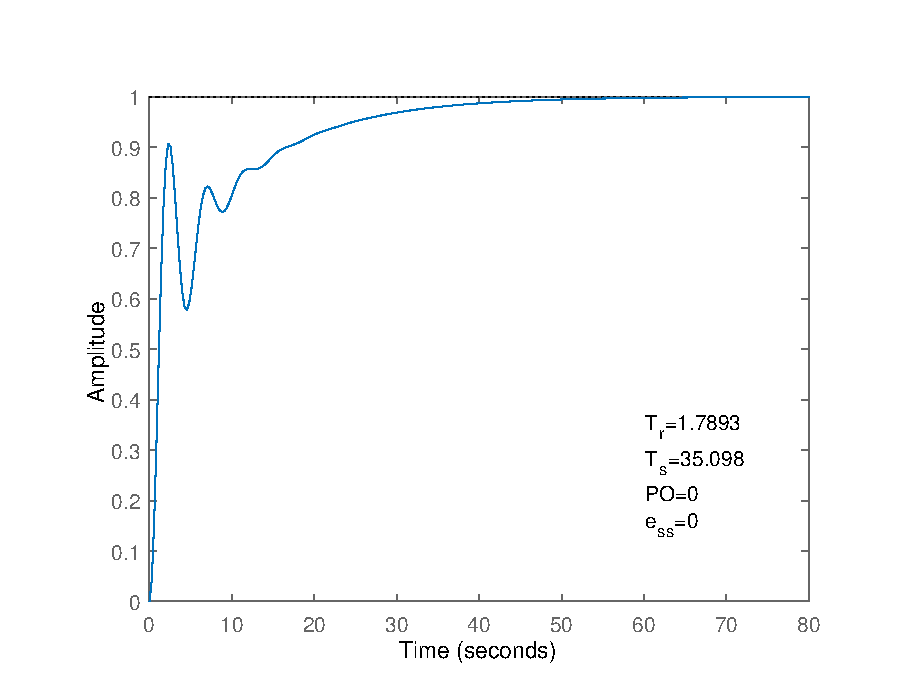
\includegraphics[scale=.5]{UncompensatedResponse.eps}
            \caption{Uncompensated Step Response}
            \label{fig:UnResp}
        \end{minipage}
    \end{figure}
    \subsection{P-Controller Closed-Loop System}
    We consider again the system in a negative feedback loop, this time with a pure proportional controller, \(G_c(s) = K\). 
    To aid analytical determination of a good K value, the region of the imaginary plane that corresponds to our requirements will be found.
    To find this region, first \(\zeta\) is determined from the required percent overshoot and given by the following
    \begin{equation}
        \begin{aligned}
            \zeta=&\sqrt{\frac{ln(PO)^2}{\pi^2+ln(PO)^2}}\\
            \zeta\approx& 0.59116
        \end{aligned}
    \end{equation}
    With $\zeta$ determined, $\theta$ is calculated
    \begin{equation}
        \begin{aligned}
            \theta=& arcos(\zeta)\\
            \theta\approx& 53.761\degree
        \end{aligned}
    \end{equation}
    $\omega_n$ is also found
    \begin{equation}
        \begin{aligned}
            \omega_n\approx& \frac{4}{\zeta T_s}\\
            \omega_n\approx& 0.67664
        \end{aligned}
    \end{equation}
    Note that \(\omega_n\) may also be determined from $T_r$, however the value of \(\omega_n\) turns out to be larger and so we choose \(\omega_n\) to be the more restrictive value calculated from $T_s$.
    The desired region is the sector with radius $\omega_n$ bounded between $\pm\theta$ as in Figure \ref{fig:PRLocus}.
    \begin{figure}[ht]
        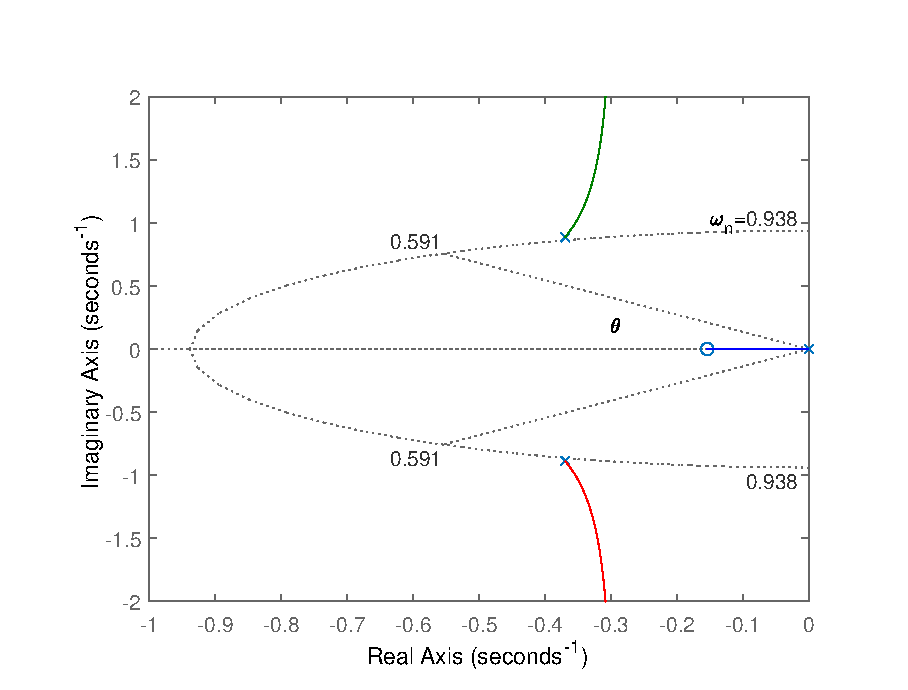
\includegraphics[scale=.5]{PRLocus.eps}
        \caption{Root Locus With Region of Interest}
        \label{fig:PRLocus}
    \end{figure}
    All of the possible locations of the poles with the given controller can be seen.
    There are no pole locations along the branches which meet the design requirements.
    To fulfill the design requirements, the shape of the root locus must be changed so that the poles of the system may fall within the space determined by the requirements.
    The root locus will be changed later with PI and PID controllers.
    However, the proportional controller does give some control over the response characteristics.
    Adjusting the gain value of K will move the poles of the system along the branches of the root locus.
    K is determined by noting the step response while K is varied with an aim of minimizing the response characteristics.
    A value of 
    \begin{equation}
        \begin{aligned}
            K&=1.5
        \end{aligned}
    \end{equation}
    is a good solution.
    This solution meets the design requirements for $T_r$, $PO$, and $e_{ss}$. 
    This plant, in a negative feedback configuration, will always have zero steady state error because it is a type one system.
    \begin{figure}[ht]
        \centering
        \begin{minipage}[t]{.5\textwidth}
            \includegraphics[scale=.5]{PPoles.eps}
            \caption{P Controller Pole-Zero Map}
        \end{minipage}%
        \begin{minipage}[t]{.5\textwidth}
            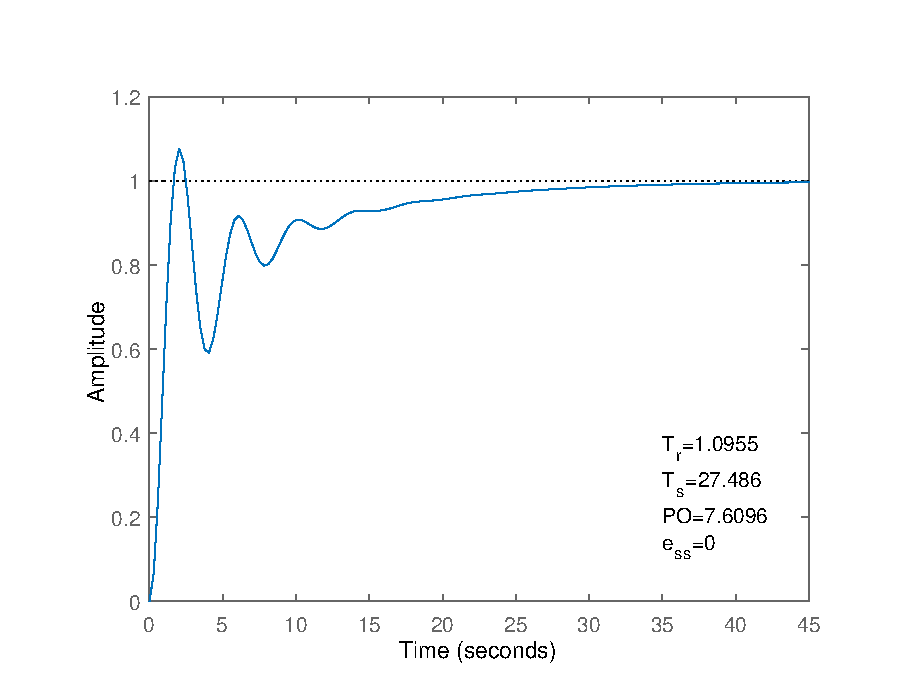
\includegraphics[scale=.5]{PResponse.eps}
            \caption{P Controller Step Response}
        \end{minipage}
    \end{figure}
    \subsection{PI-Controller Closed-Loop System}
    The same system is studied, this time with controller $G_c(s)=K_P+\frac{K_I}{s}$.
    The gain values are found again by manually tuning. 
    P and I are adjusted until the step response characteristics are approximately minimized.
    The designed controller has the following gains.
    \begin{equation}
        \begin{aligned}
            &K_P=0.4\\
            &K_I=0.3
        \end{aligned}
    \end{equation}
    The poles and step response are in figures \ref{fig:PIPoles} and \ref{fig:PIResponse} respectively.
    \begin{figure}[ht]
        \centering
        \begin{minipage}[t]{.5\textwidth}
            \includegraphics[scale=.5]{PIPoles.eps}
            \caption{PI-Controller Pole-Zero Map}
            \label{fig:PIPoles}
        \end{minipage}%
        \begin{minipage}[t]{.5\textwidth}
            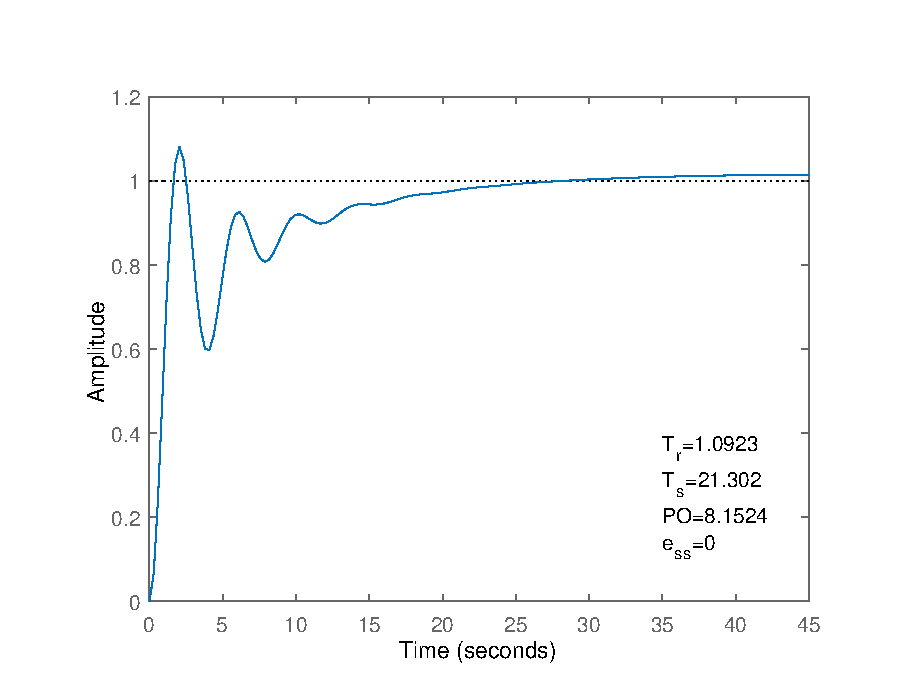
\includegraphics[scale=.5]{PIResponse.eps}
            \caption{PI-Controller Step Response}
            \label{fig:PIResponse}
        \end{minipage}\hfill
    \end{figure}
    This solution meets the design requirements for $T_r$, $PO$, and $e_{ss}$.
    This response is very similar to the P-controller, the plant already has an integrator so adding another is not much help.
    \subsection{PID-Controller Closed-Loop System}
    We now consider the controller $G_c(s)=K_P+\frac{K_I}{s}+K_Ds$.
    The tuning procedure followed is similar to that for the PI controller. 
    The PID gains are manually adjusted until the requirements are met.
    The D gain is then lowered until the response characteristics barely meet the requirements.
    Keeping the D gain low will improve the noise rejection of the controller.
    The controller has the gains as given.
    \begin{equation}
        \begin{aligned}
            &K_P=7\\
            &K_I=7\\
            &K_D=5
        \end{aligned}
    \end{equation}
    The controller's graphs are in figures \ref{fig:PIDPoles} and \ref{fig:PIDResponse}.
    \begin{figure}[ht]
        \centering
        \begin{minipage}[t]{.5\textwidth}
            \includegraphics[scale=.5]{PIDPoles.eps}
            \caption{PID-Controller Pole-Zero Map}
            \label{fig:PIDPoles}
            \end{minipage}%
        \begin{minipage}[t]{.5\textwidth}
            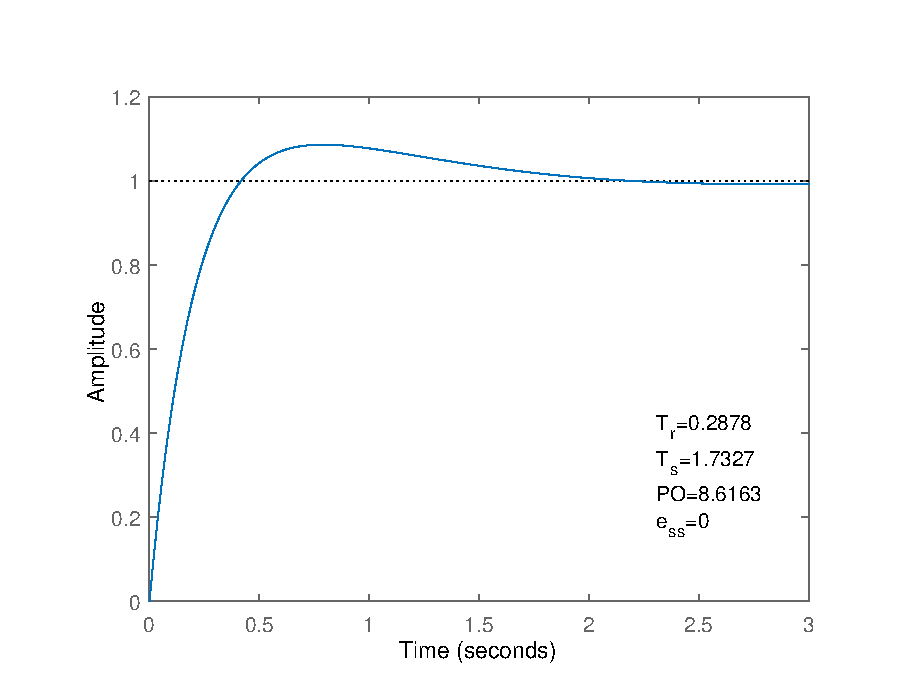
\includegraphics[scale=.5]{PIDResponse.eps}
            \caption{PID-Controller Step Response}
            \label{fig:PIDResponse}
        \end{minipage}\hfill
    \end{figure}
    This solution meets all the design requirements.
    The PID controller is the only studied controller which meets all the design requirements.
    \section{Problem 2}
    \subsection{Background and Research}
    Magnetic Levitation is a system in which a vehicle is levitated above a track or rail while still following the path of the track using electromagnetic forces. There are superconducting magnets on the vehicle and coils on the pathway.
    When you place two magnets of the same polarity near each other, they repel each other. If you place them on top of each other the result is that one is levitated temporarily due to the repulsion force.
    Earnshaw's Theorem tells us there is no such equilibrium point in a static electric field to create stable levitation. This is solved by using an electromagnet, where the magnetic field is not static.

    \subsection{Problem Definition}
    Given the magnetic levitation system in Figure \ref{fig:CircuitDiagram}, we are asked to derive the governing equations.
    \begin{figure}[ht]
        \makebox[0pt]{\documentclass[border = .2cm]{standalone}
\usepackage{circuitikz}

\def\dx{0.3}
\def\dy{0.3333}
\def\x{0}
\def\xx{1}
\def\y{3}

\begin{document}
\begin{circuitikz}[american voltages]
\draw
  (1,0) to [L, l_=$L$] (3,0)
  to [short] (4,0)
  to [V, l_=$e(t)$, invert] (4,3) 
  to [R, l_=$R$] (0,3);
\draw 
    (3.1,3) to [short,i=$I$] (3,3);
\draw
    (4,0) node[ground]{};
\draw[fill=blue!20,] (0,-.4)rectangle(1,3.4);
\node at (.5,0){M};
\foreach \i in {0,2,4,6}
{	
    \draw (\x,\y-\i*\dy) ..controls (\x-\dx, \y-\i*\dy) and (\x-\dx,\y-\dy-\i*\dy).. (\x,\y-\dy-\i*\dy);
    
    \draw (\xx,\y-\i*\dy-\dy) ..controls (\xx+\dx, \y-\i*\dy-\dy) and (\xx+\dx,\y-\i*\dy-2*\dy).. 
                        (\xx,\y-\i*\dy-2*\dy);
                        
    \draw (\xx,\y-\i*\dy) -- (\x,\y-\i*\dy);
    
    \draw (\x,\y-\i*\dy-2*\dy) ..controls (\x-\dx, \y-\i*\dy-2*\dy) and (\x-\dx,\y-\dy-\i*\dy-2*\dy).. (\x,\y-\dy-\i*\dy-2*\dy);
    
    \draw (\xx,\y-\i*\dy-2*\dy) -- (\x,\y-\i*\dy-2*\dy);

}
\draw[->] (-1,-.5)--(-1,-1) node[below]{$x$};
\draw (-1.2,-.5)--(-.8,-.5);

\draw[->] (-1,2)--(-1,1.5) node[below]{$g$};
\draw (-1.2,2)--(-.8,2);

\end{circuitikz}
\end{document}}
        \caption{Magnetic Levitation System}
        \label{fig:CircuitDiagram}
    \end{figure}
    where  M is mass, v is velocity, x is position, k is a physical constant, I is current,
    L is inductance, R is resistance, g is gravity, and e is input voltage.
    \begin{equation}\nonumber
        \begin{aligned}
            &M=0.068 kg\\
            &k=3.2654\times10^{-5}\\
            &L=0.4125 H\\
            &R=10 \Omega
        \end{aligned}
    \end{equation}
    \subsection{Deriving the governing equations}
    We derive the equations governing the system for the magnetic levitation system.
    \begin{align} 
        \label{eqn:lev1}
        \frac{d}{dt}(x(t))&=v(t)\\
        \label{eqn:lev2}
        M\frac{d}{dt}(v(t))&=Mg-k\frac{I^2(t)}{x^2(t)}\\
        \label{eqn:lev3}
        L\frac{d}{dt}(I(t))&=-RI(t)+e(t)
    \end{align} 
    Equation (\ref{eqn:lev1}) is the derivative of position - velocity.
    Equation (\ref{eqn:lev2}) is the force experienced by the ball F = Ma.
    The derivative of the velocity is acceleration.
    Mg is the force due to gravity that will pull it downwards.
    The force acting against the force due to gravity is the magnetic force from the coil.  
    Equation (\ref{eqn:lev3}) is a KVL around the circuit.
    The voltage through an inductor is equivalent to the inductance times the derivative of the current. The voltage through a resistor is equivalent to the resistance times the current.  
    \begin{equation}
        e(t) = RI(t) + L\frac{di}{dt}(I(t))
    \end{equation}
    \subsection{Determining the equilibrium state variables}
    We determine the equilibrium state variables for a constant input voltage with magnitude $e = 24 V$ and determine a set of first-order linearized differential equations describing the system dynamics.
    To start to find the equilibrium, the left side of each equation is set to zero. This is the result
    \begin{equation}
        \begin{aligned}
            &\bar{v} = 0\\
            &\bar{I} = \frac{\bar{e}}{R}=\frac{E}{R}\\ 
            &\bar{x} = \sqrt{k/(Mg)}\bar{I} = \frac{e\sqrt{k/(Mg)}}{R}\\
        \end{aligned}
    \end{equation}
    Linearize the set
    \begin{equation}
        \begin{aligned}
            &\frac{dx}{dt} = v &= f1\\
            &\frac{dv}{dt} = g - \frac{kI^2}{Mx^2} &= f2\\
            &\frac{dI}{dt} = -\frac{R}{L}I + \frac{1}{L}e &= f3 \\
        \end{aligned}
    \end{equation}
    After doing the Taylor Series Expansion, we have  
    \begin{equation}
        \begin{aligned}
            \dot{\tilde{x}}&=\tilde{v}\\
            \dot{\tilde{v}}&=\frac{2k\bar{I}^2}{m\bar{x}^3}\tilde{x}-\frac{2k\bar{I}}{m\bar{x}^2}\tilde{I}\\
            \dot{\tilde{I}}&=-\frac{R}{L}\tilde{I}+\frac{1}{L}\tilde{e}
        \end{aligned}
    \end{equation}
    where
    \begin{equation}
        \begin{aligned}
            \tilde{x}&=x-\bar{x}\\
            \tilde{v}&=v-\bar{v}\\
            \tilde{I}&=I-\bar{I}\\
            \tilde{e}&=e-E
        \end{aligned}
    \end{equation}
    Next, let's substitute our values in for our variables.
    \begin{equation}
        \begin{aligned}
            \dot{\tilde{x}}&=\tilde{v}\\
            \dot{\tilde{v}}&=\frac{2(3.2654\times10^{-5})\bar{I}^2}{(0.068kg)\bar{x}^3}\tilde{x}-\frac{2(3.2654\times10^{-5})\bar{I}}{(0.068kg)\bar{x}^2}\tilde{I}\\
            \dot{\tilde{I}}&=-\frac{10\Omega}{0.14125H}\tilde{I}+\frac{1}{0.4125}\tilde{e}
        \end{aligned}
    \end{equation}
    Which becomes
    \begin{equation}
        \begin{aligned}
            \dot{\tilde{x}}&=\tilde{v}\\
            \dot{\tilde{v}}&=-84.4\tilde{I}+84.4\tilde{x}\\
            \dot{\tilde{I}}&=-70.8\tilde{I}+2.42\tilde{e}
        \end{aligned}
    \end{equation} 
    Taking the Laplace transform of our equations
    \begin{equation}
        \begin{aligned}
            Xs^2=&84.4X-84.4I\\
            Is=&-70.8I+2.42E\\  
        \end{aligned}
    \end{equation} 
    and solving for the transfer function $G=\frac{X(s)}{E(s)}$ we have
    \begin{equation}
        \begin{aligned}
            G = \frac{204.25}{s^3+70.8s^2-84.4s-5976}
            \label{eqn:levTrans}
        \end{aligned}
    \end{equation}
    \subsection{Designing a controller}
    A controller is designed for the linearized system to stabilize it about its equilibrium.
    The linearized transfer function in (\ref{eqn:levTrans}) is used.
    Graphing in MatLab's Control System Designer, we start with a lead compensator - where the pole is closer to the origin than the zero.
    By manually adjusting the compensator, the goal of stabilizing the system is met.
    The designed controller is
    \begin{equation}
        \begin{aligned}
            G_c = \frac{1615.6}{(s+7)(s+100)}
        \end{aligned}
    \end{equation}
    where the pole is located at s=-100 and the zero at -7.
    The step response of the closed-loop linearized system is in Figure \ref{fig:LevResponse}. The theoretical implementation of the controller on the non-linear system is not explored.
    \begin{figure}[ht]
        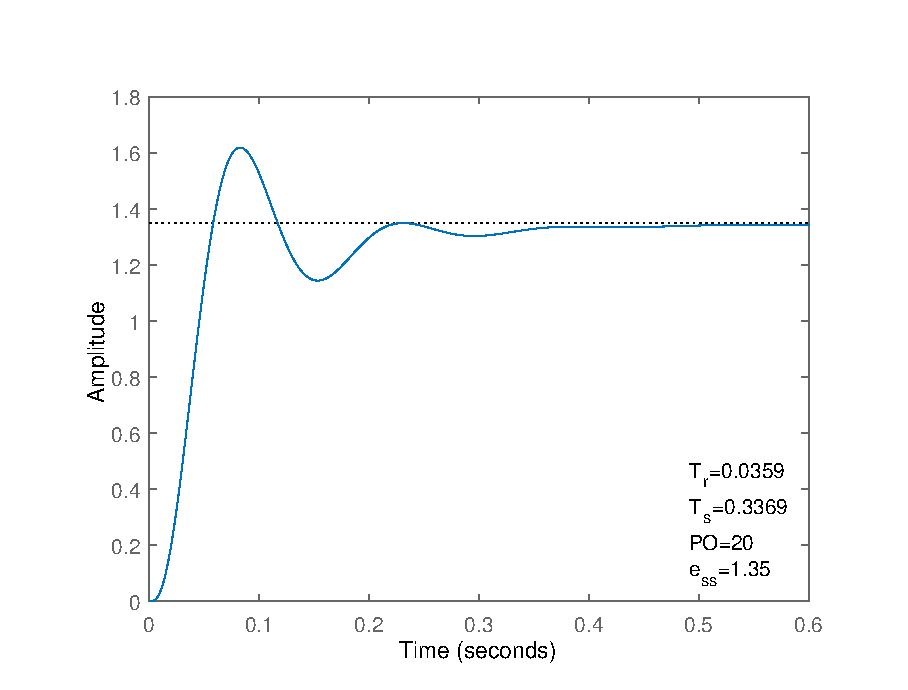
\includegraphics[scale=.5]{LevResponse.eps}
        \caption{Linearized System Step Response}
        \label{fig:LevResponse}
    \end{figure}
\end{document}